\chapter{はじめに}
被災地での救助活動を行う際に,人間の補助として訓練されたレスキュー犬(災害救助犬)が探査を行う場合がある.レスキュー犬は,犬としての特性を生かして人間と協力して被災地の探索を行う.がれきの隙間などの狭い空間,倒壊した建物など人間には踏破困難な環境でも探査可能であり,また発達した嗅覚を頼りにした救助活動が可能である.しかし,彼らは人間に向けた言語を持たないため,人間はレスキュー犬の行動から彼らが収集した情報を理解しなくてはならない.現状では,レスキュー犬を指揮するハンドラーと呼ばれる人間がレスキュー犬の行動を手動でマーキングしており,その情報を消防などの指揮命令者に口頭伝達している.このレスキュー犬との共同探索の問題点として,トリアージ(緊急度に従った手当の優先順位付け)のための周辺環境情報や,要救助者情報の不足があげられる.また,ハンドラーによる記録はどうしても主観的になり客観性が不足し,さらにそれを口頭伝達することで正確性がより不足する.

本研究では,レスキュー犬にセンサを装着して得られたデータ用いてレスキュー犬の行動をリアルタイムに分類すること目的とする.深層学習を用いた画像識別にある既存手法を予備実験として行った.予備実験をもとに,動画からのレスキュー犬行動分類を行う.本研究は映像だけでなく音声などのデータも活用したマルチモーダルな動画分類である.本研究により,レスキュー犬が今何をしているのか明示的に判断することが可能となり,トリアージに必要な情報が整理され,災害救助活動の効率化が期待される.

\chapter{関連研究}

レスキュー犬の行動をモニタリングするために,濱田,大野らによって装着型計測・記録装置が開発された~\cite{dog01}.図\ref{cyber}にレスキュー犬に装着可能な軽量な行動計測スーツ示す.これを着用したレスキュー犬はサイバー救助犬とも呼ばれる.各種センサを用いた計測データを記録し,リアルタイムに映像などのデータを無線配信することが可能である.そのため,レスキュー犬が人の目の及ばない範囲で活動する際にもレスキュー犬の行動やその周辺環境などを把握するのに役立つ.サイバー救助犬は,政府による総合科学技術・イノベーション会議が研究開発を促進しているImPACTというプログラムのタフ・ロボティクス・チャレンジの一環である.
タフ・ロボティクス・チャレンジとは災害救助を目的としたロボットの研究開発プロジェクトであり,その中で,災害救助用サイボーグ犬の開発の足掛かりとしてサイバー救助犬が研究されている.

\begin{figure}[htbp]
 \begin{center}
  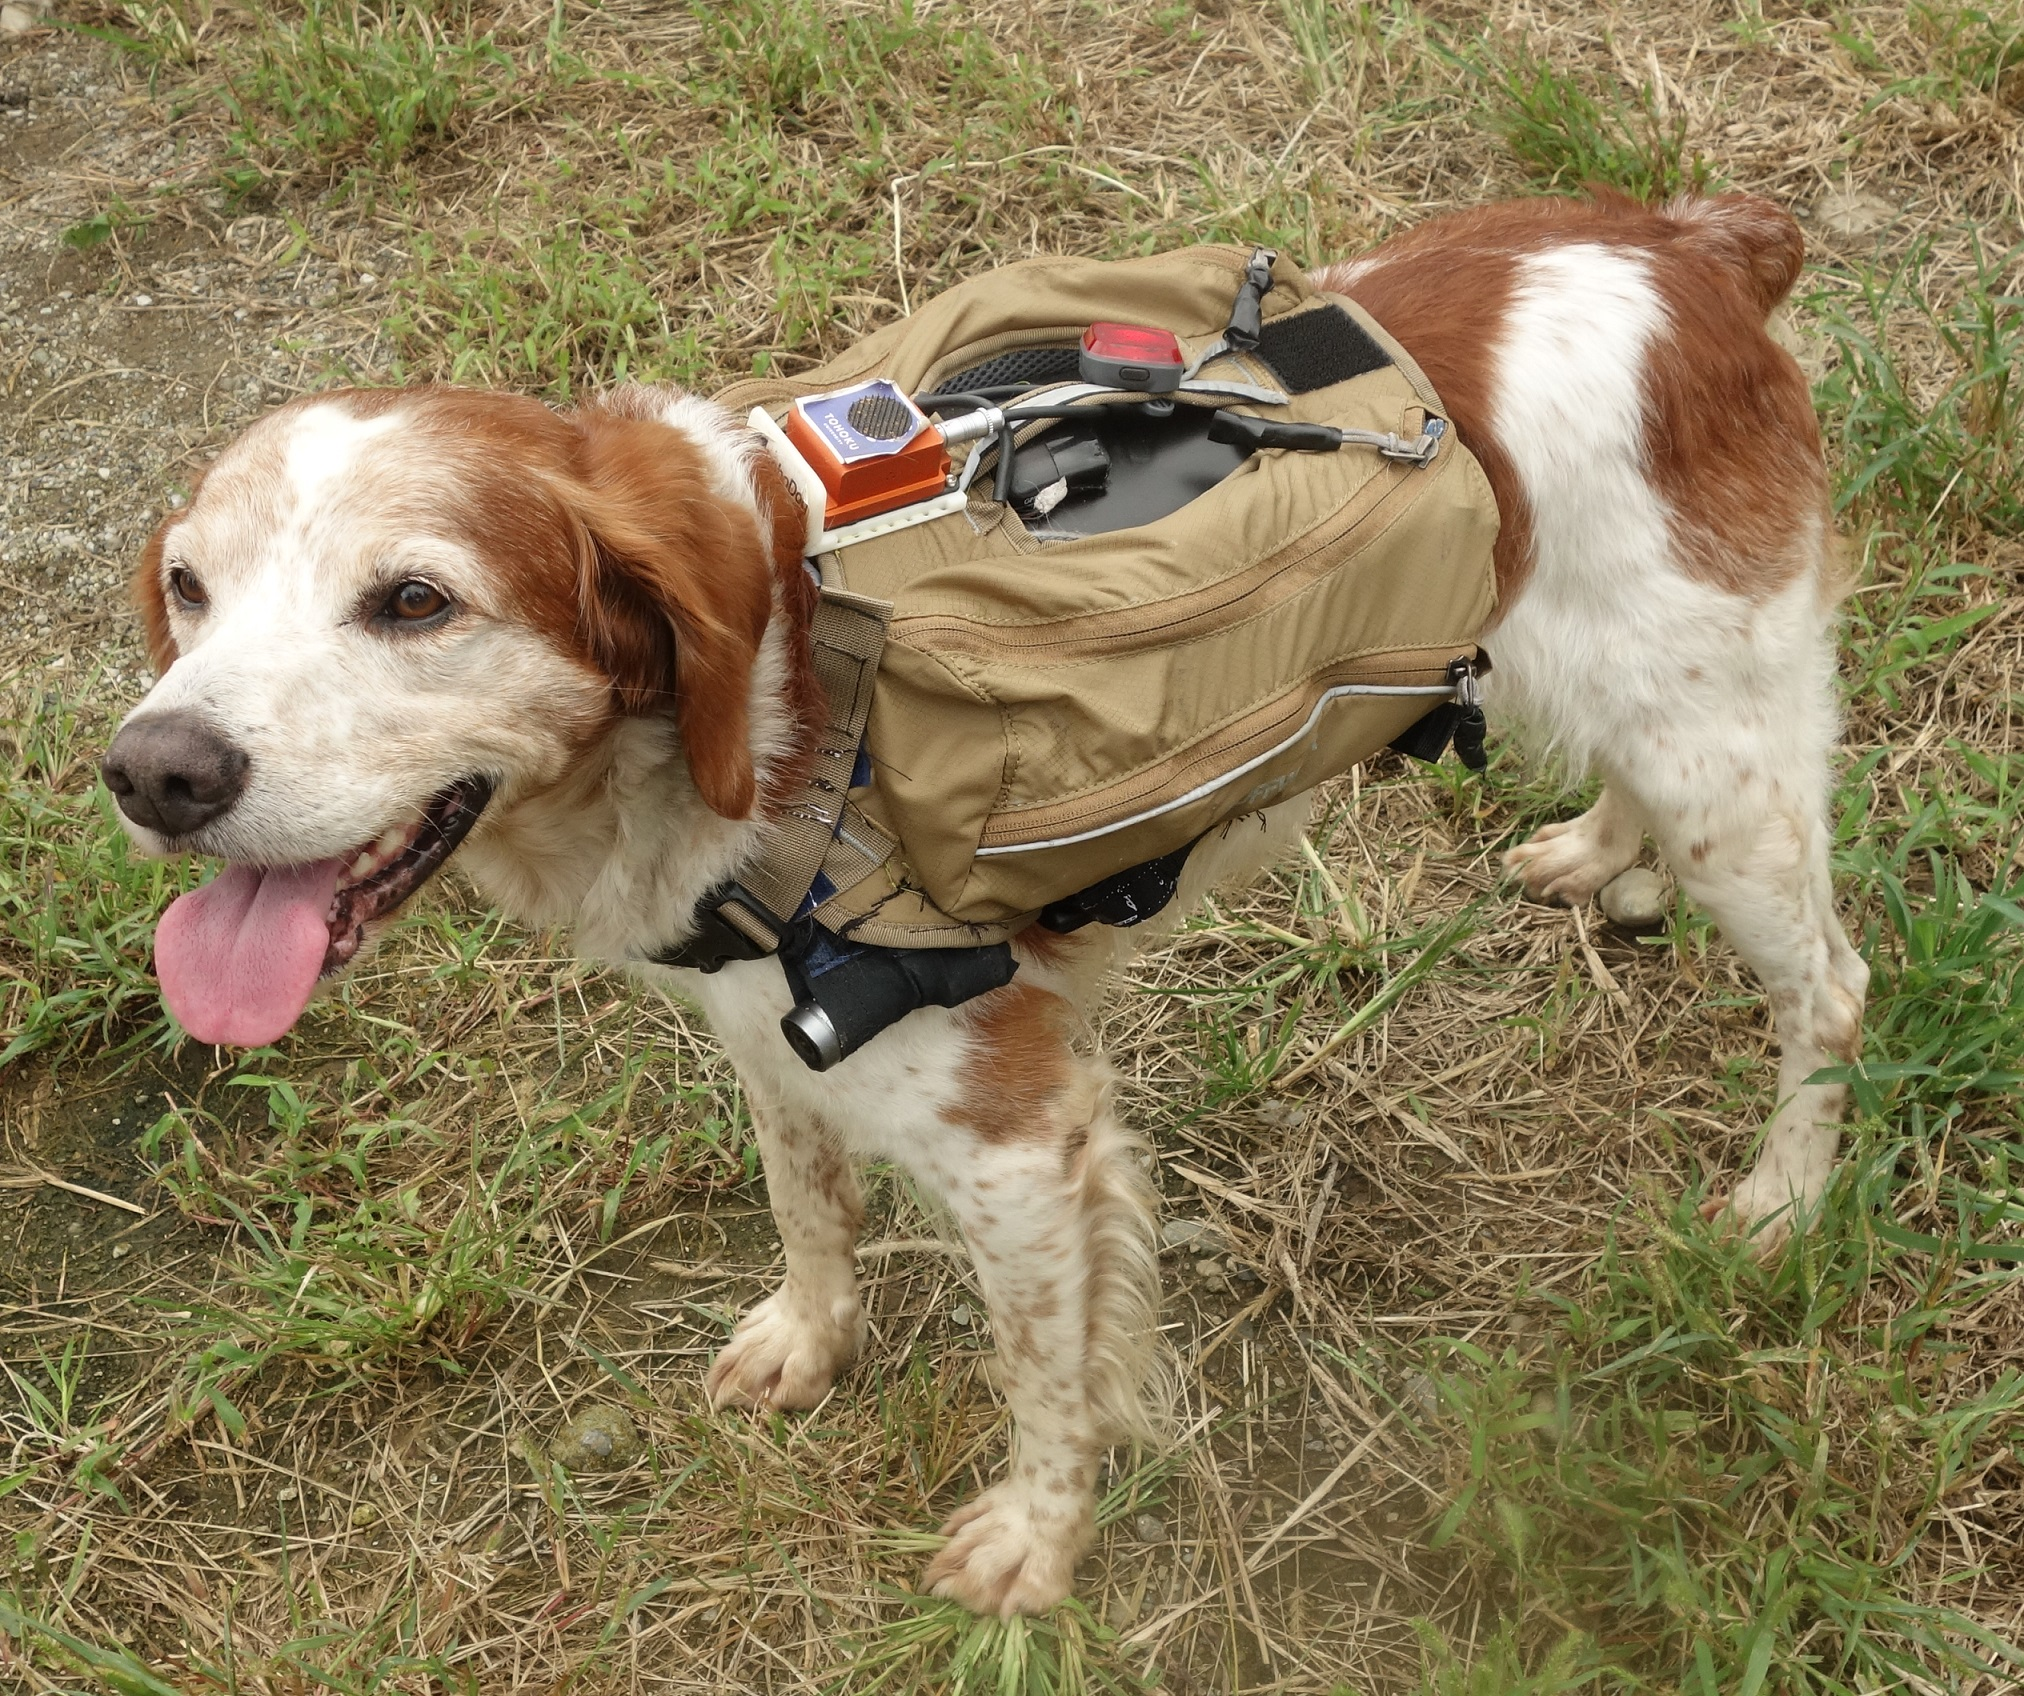
\includegraphics[width=6cm]{./Figures/cyberdog.eps}
  \caption{装着型計測・記録装置~\cite{dog01}より引用}
  \label{cyber}
 \end{center}
\end{figure}

また,Ehsanらによる犬の一人称視点動画からの犬行動予測の研究がある~\cite{whoretthedog}.これは,犬の行動をモデリングし,犬が次にどのような道をたどり行動するかを予測している.

%\section{問題点}
しかし,これらの研究は犬の行動のモデリングであり,犬の周辺環境の推定などは行っていない.また,入力は動画像のみであり,音声などのデータは利用していない.レスキュー犬の課題には,犬の周辺環境情報や動画像からだけでは判断できない情報の取得が含まれている.例えばレスキュー犬は要救助者を発見するとその場で待機し吠え続けるように訓練されている.このように,動画像データからだけではなく,音声データ,および慣性データ・GPSデータなどの情報を複合的に用いてレスキュー犬の状態を判断しなければならない.本研究は動画像と音声からなるマルチモーダルな情報を入力とした犬の行動の分類を目的としている. 

